\chapter{Estimating Feature Saliency Using 2D Saliency Maps \label{2d_saliency_map}}

A saliency map is a model of visual attention using bottom-up features such as intensity, color and orientation of an image.
In order to use 2D saliency maps \cite{itti_model_1998} to estimate visual saliency of 3D features in volume visualization, an inverse distance weighting \cite{shepard_two-dimensional_1968} can be applied to divide a 2D saliency map into several feature saliency maps, one for each feature. Subsequently, the visual saliency of each feature can be estimated with the total intensity of each feature saliency map.

%The distance between a pixel of each feature and the pixel in the final image is necessary in computing the inverse distance weighting.
We render an image $ P_{i} $ of each feature separately with the same settings (viewpoint, screen size etc.) as the final image and compute a saliency map $ S $ of the final image.
Let $ w_{i} $ be the weight of a pixel $ p $ in the $i$-$th$ feature
\[ w_{i} = \frac{ \frac{1}{d_{i}^{m}} }{ \sum_{j=1}^{n} \frac{1}{d_{j}^{m}} } \]
where $ d_{i} $ is the color distance between the pixel $ p $ in the final image and the corresponding pixel $ p_{i} $ in the $i$-$th$ feature image.
$ n $ is the number of features.
$ m $ is a user-defined coefficient for controlling the bias of the weighting. Pixels with small distances would have larger weights when $ m $ increases. $ m=1 $ is used and the color distance $ d_{i} $ is computed in the LAB color space in our implementation

Then the corresponding pixel $ s_{i} $ in the $i$-$th$  feature saliency map is
\[ s_{i}=w_{i}s \]
where $ s $ is the pixel in the 2D saliency map $ S $ of the final image.

Therefore, we can obtain $ n $ feature saliency maps by performing the above a pixel-wise operation using the 2D saliency map $ S $ and the final image $ P $ along with each feature images $ P_{i} $ respectively.

Figure~\ref{fig:engine_naive} shows an engine block ($ P $) and its two features ($ P_{1} , P_{2} $).
Figure~\ref{fig:engine_naive_saliencemap} shows the 2D saliency map $ S $ and the two feature saliency maps($ S_{1} , S_{2} $) obtained using the above operation.
The saliency maps in Figure~\ref{fig:engine_naive_saliencemap} are enhanced (multiplied by 8) for better contrast in illustrations. The original saliency maps are used in our implementation.

After dividing the 2D saliency map $ S $ into feature saliency maps with the inverse distance weighting, there are a small amount of bright pixels (around the boundary of the engine block) left in the 2D saliency map $ S $, as shown in Figure~\ref{fig:engine_naive_saliencemap_features}~(a). Let this left saliency image be $ S' $.
We divide these values and add them to the feature saliency maps using another weighting with the Gaussian of the current feature saliency maps.
Firstly, we apply a Gaussian filter with kernel size $ k $ to each feature saliency map $ S_{i} $ and get the Gaussian image $ G_{i} $.
The kernel size $ k $ should be large in order to allow the resulting Gaussian image to have non-zero pixels to cover the bright pixels in the left saliency image $ S' $.
Let $ g_{i} $ be a pixel in the Gaussian image $ G_{i} $.
Secondly, we divide the left saliency image $ S' $ into $ n $ images ($ S'_{1} $ ... $ S'_{n} $).
%\[ G_{i}=Gaussian(S_{i},k) \]
\[ s'_{i} = \frac{ g_{i} }{ \sum_{j=1}^{n} g_{j} }s' \]
where $ s' $ is a pixel in $ S' $.

Finally, we pixel-wisely add the image $ S'_{i} $ to the feature saliency map $ S_{i} $ and obtain the final feature saliency map.
\[ T_{i} =S_{i}+S'_{i}\]

Figure~\ref{fig:engine_naive_saliencemap_features}~(b) and (c) respectively display the final feature saliency maps of the red feature and the green feature of the engine block.

\begin{figure}
	\centering
	\begin{minipage}{.33\textwidth}
		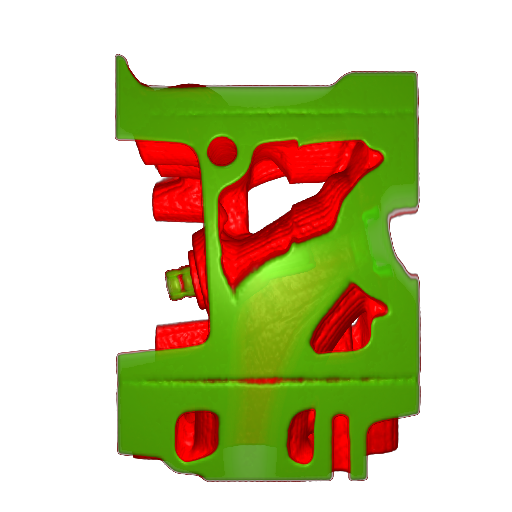
\includegraphics[width=1\linewidth]{images/engine_naive}
		\subcaption{}
	\end{minipage}~
	\begin{minipage}{.33\textwidth}
		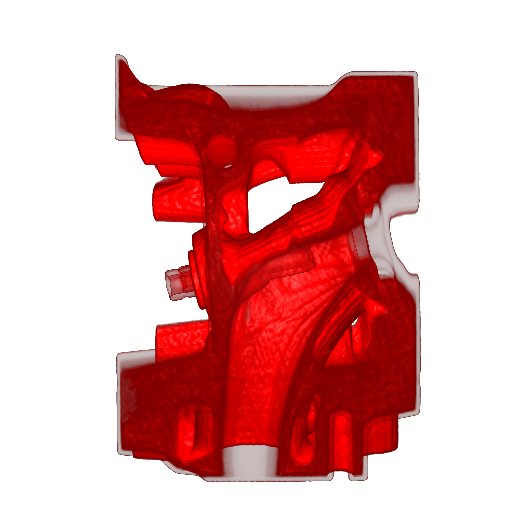
\includegraphics[width=1\linewidth]{images/engine_naive_1}
		\subcaption{}
	\end{minipage}~
	\begin{minipage}{.33\textwidth}
		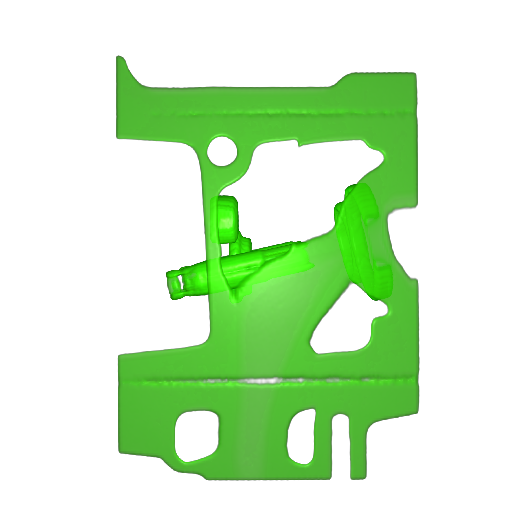
\includegraphics[width=1\linewidth]{images/engine_naive_2}
		\subcaption{}
	\end{minipage}
	\caption{An engine block (a) and its red feature (b) and green features (c) respectively}
	\label{fig:engine_naive}
\end{figure}

\begin{figure}
	\centering
	\begin{minipage}{.33\textwidth}
		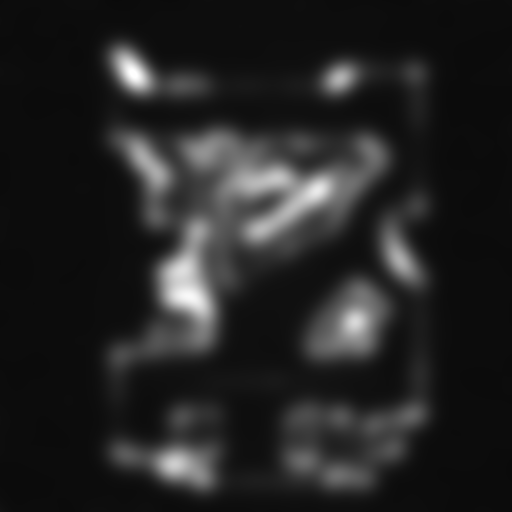
\includegraphics[width=1\linewidth]{images/engine_naive_saliencemap}
		\subcaption{}
	\end{minipage}~
	\begin{minipage}{.33\textwidth}
		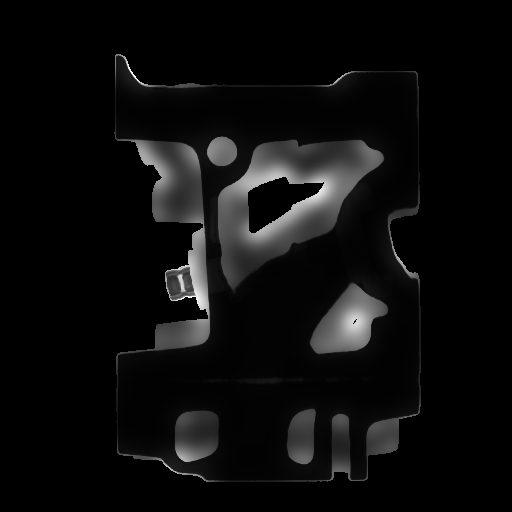
\includegraphics[width=1\linewidth]{images/engine_naive_saliencemap_1_overlap}
		\subcaption{}
	\end{minipage}~
	\begin{minipage}{.33\textwidth}
		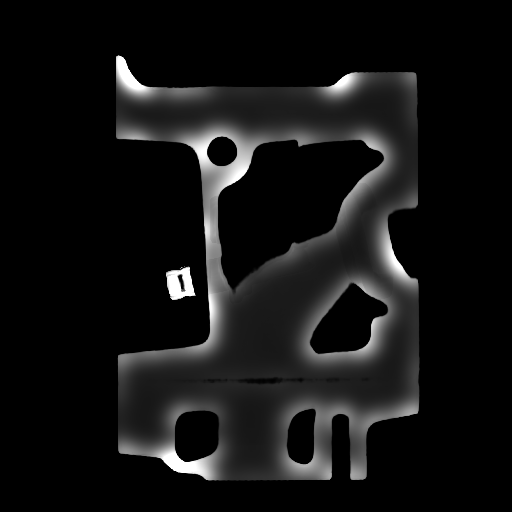
\includegraphics[width=1\linewidth]{images/engine_naive_saliencemap_2_overlap}
		\subcaption{}
	\end{minipage}
	\caption{2D saliency maps (a) and the two feature saliency maps (b) and (c). The saliency maps are enhanced (multiplied by 8) for better contrast in illustrations.}
	\label{fig:engine_naive_saliencemap}
\end{figure}

\begin{figure}
	\centering
	\begin{minipage}{.33\textwidth}
		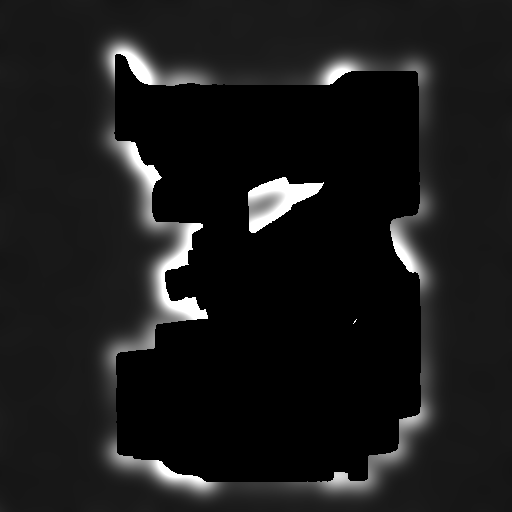
\includegraphics[width=1\linewidth]{images/engine_naive_saliencemap_left}
		\subcaption{}
	\end{minipage}~
	\begin{minipage}{.33\textwidth}
		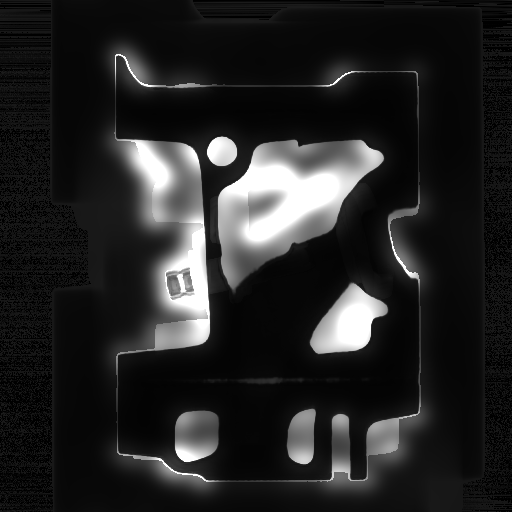
\includegraphics[width=1\linewidth]{images/engine_naive_saliencemap_1}
		\subcaption{}
	\end{minipage}~
	\begin{minipage}{.33\textwidth}
		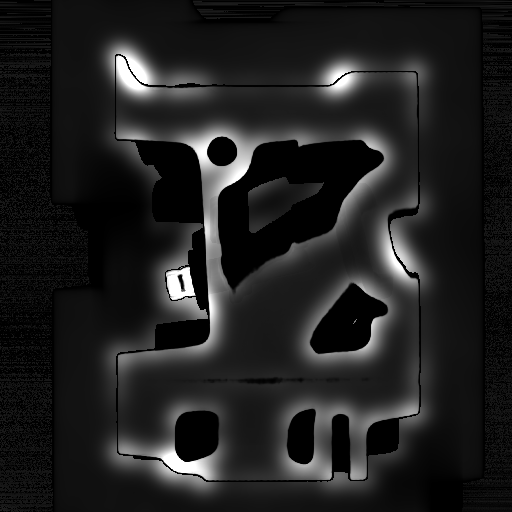
\includegraphics[width=1\linewidth]{images/engine_naive_saliencemap_2}
		\subcaption{}
	\end{minipage}
	\caption{Values left in the 2D saliency map (a) and the two final feature saliency maps (b) and (c) after adding the values left in (a)}
	\label{fig:engine_naive_saliencemap_features}
\end{figure}

